
\documentclass[10pt,a4paper]{article}

% formatting requires ecua.sty style file 
\usepackage{ecua}
% load some other useful packages
\usepackage{cite} % improved formatting for citation lists
\usepackage{graphicx}

\title{\textrm{\LaTeX} template for the 11th European Conference on Underwater Acoustics, ECUA 2012 [max. 3 lines for title, left justified]}

% please edit the following tabular environment
% for \author block to match conference formatting
% use & to separate author and institution
% end each author line with \\
\author{%
\begin{tabular}{p{30mm}p{125mm}}
AN Author & Institute of Acoustics, St Albans, Herts., UK \\
AN Other &  Dept. of Electrical \& Electronic Engineering, Loughborough University of Technology, Loughborough, UK\\
D Bird & Cricket Acoustics Ltd., Dolphinston, Roxburghshire, UK \\
\end{tabular}
}

\begin{document}

\maketitle

\section{Introduction}
This document provides formatting suitable for paper submissions to ECUA 2012. It uses package ecua.sty available by separate download from the conference website. In case of difficulty in obtaining the style file or to report bugs or deficiencies please contact c.capus@hw.ac.uk. Some good references for help in using \textrm{\LaTeX} are listed below\cite{kopka:latex, goosens:latex, pakin:latexSymbols}.

\section{Formatting [Section Headers are set in Uppercase `L\MakeLowercase{arge}'  type, 14pt size]}
This exemplifies the section heading style. For specific cases where lowercase is needed for understanding, as above, it can be forced using the command \textbackslash\texttt{MakeLowercase}\{\texttt{text to be set in lowercase}\} --- this can also be applied in the paper title and subsection headers if required.

\subsection{[Subsection Headers are set in Uppercase `\MakeLowercase{large}'  type, 12pt size]}
This exemplifies the subsection heading style.

\subsubsection{[Subsubsection Headers are Set in `\MakeLowercase{large}' Type, 12pt Size]}
This exemplifies the subsubsection heading style, which should be set in titlecase --- that is, capitalise only the first letter of each word. Further heading levels are strongly discouraged.

\subsection{Main body text}
Main body text is typeset in 10pt Helvetica sans serif font with single spacing. Page margins are set at: left 27mm; right 27mm; bottom 30mm; top 40mm on title page and 30mm on subsequent pages. Text should be fully justified.

Do not include any page numbers. These will be added by the typesetters once all of the papers have been collated.

\subsection{Headers and Footers}
Every page shall carry the header: Proceedings of the 12th European Conference on Underwater Acoustics. Every page shall carry the footer: Vol. XX. Pt. Y 2009. The volume and part numbers will be provided by the conference organisers.  All headers and footers are left justified and set in bold type.

\section{Tables and Figures}

Tables and Figures are set in the floating table and figure environments. Table and Figure positioning is suppressed at the top of the first page.

\subsection{Figures}

The graphics and graphicx packages are recommended for Figure placement, an example is given in Figure~\ref{fig1:egFig}. The caption is included below the Figure.

\begin{figure}
\begin{center}
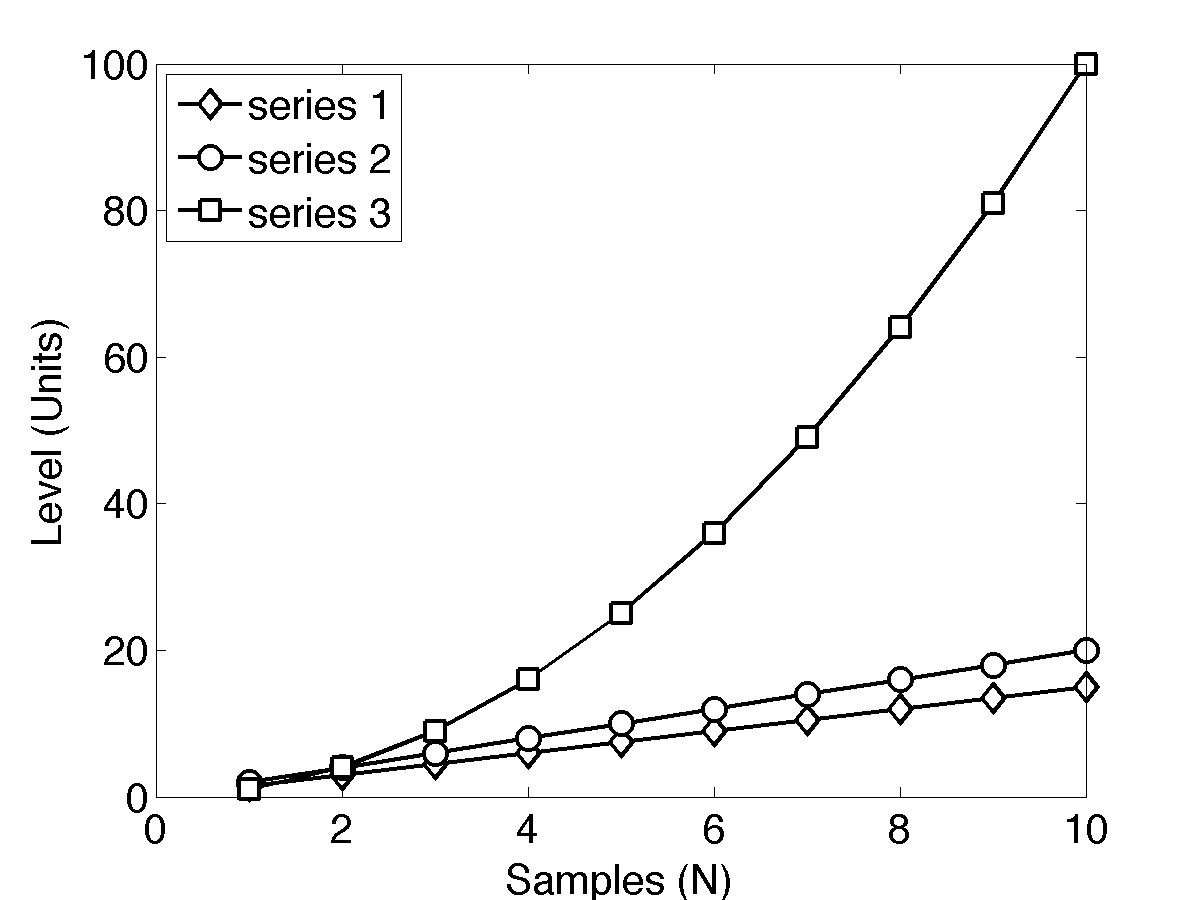
\includegraphics[width=10cm]{./egFigure.png}
\caption{\label{fig1:egFig} Example graph -- please avoid unnecessary use of colour and ensure line and marker styles allow discrimination when printed or copied in black and white}
\end{center}
\end{figure}

\subsection{Tables}
Tables are included using the tabular environment within a table float. An example is given in Table~\ref{tab1:egTable}. At the authors' discretion, entries in the titles line may be set in bold type, as in this example. The caption is included below the Table.

\begin{table}[h]
%\renewcommand{\tabcolsep}{1em}
\begin{center}
\begin{tabular}{|r|rrr|}
\hline
\textbf{X value} & \textbf{Y1 value} & \textbf{Y2 value} & \textbf{Y3 value} \\
\textbf{(units)} & \textbf{(units)} & \textbf{(units)} & \textbf{(units)} \\
\hline
1 & 2 & 1.5 & 1  \\
2 & 4 & 3.0 & 4  \\
3 & 6 & 4.5 & 9 \\
4 & 8 & 6.0 & 16 \\
5 & 10 & 7.5 & 25 \\
6 & 12 & 9.0 & 36 \\
7 & 14 & 10.5 & 49 \\
8 & 16 & 12.0 & 64 \\
9 & 18 & 13.5 & 81 \\
10 & 20 & 15.0 & 100 \\
\hline
\end{tabular}
\caption{\label{tab1:egTable} Example table}
\end{center}
\end{table}

\section{Other Formatting}

\subsection{Equations and Equation Numbering}

Equations are included with the equation and eqnarray environments. Numbers should appear in brackets to the right of each numbered equation line. Equation references in the text are of the form equation~(\ref{eqn1}).

\begin{equation}
\Re = \sqrt{\frac{\alpha}{\beta}}^n
\label{eqn1}
\end{equation}

\subsection{Footnotes}
Footnotes are discouraged due to the reduction in font sizes in the reprinted materials. If deemed necessary they can be included using the \textbackslash\texttt{footnote}\{\} command.\footnote{which will set in microscopically small text at the bottom of the current page if space is available.}

\subsection{Alternative Font Styles}

If required for particular emphasis, a limited number of alternative font styles can be selected as follows:

\begin{tabular}{ll}
COMMAND & RESULT \\
\textbackslash\texttt{texttt}\{\texttt{Teletype font}\} & \texttt{Teletype font} \\
\textbackslash\texttt{textrm}\{\texttt{Roman font}\} & \textrm{Roman font} \\
\textbackslash\texttt{textsc}\{\texttt{Small Caps font}\} & \textsc{Small Caps font} \\
\textbackslash\texttt{textbf}\{\texttt{Bold font}\} & \textbf{Bold font} \\
\textbackslash\texttt{textit}\{\texttt{Italic font}\}  & \textit{Italic font} \\
\textbackslash\texttt{emph}\{\texttt{Italic font}\}  & \emph{Italic font} \\
\end{tabular}

\section{Citations and References}
An ECUA \textrm{\BibTeX} style file, ecua.bst, is available from the conference website. This is based on the standard \texttt{plain} style file. Citations are made in the usual way using the \textbackslash\texttt{cite}\{\} command. Examples of various entry types can be found in the References section below: a journal article~\cite{capus:biosonar}; an article published in conference proceedings~\cite{thode:marRecord}; a book~\cite{au:dolphins}; a chapter in an edited book~\cite{abramowitz:handbook}; a fully attributed section from an edited volume~\cite{green:mcmc}; a PhD thesis~\cite{muller:bats}; a technical report~\cite{APL-UW:handbook}. 

\section*{Acknowledgements}
Any acknowledgements section should immediately precede the References with no section number. This is achieved using the starred \textrm{\LaTeX}\,tag \textbackslash\texttt{section*}\{\texttt{Acknowledgements}\}.

\bibliographystyle{./ecua}
\bibliography{ecua}

\end{document}



